\documentclass{article}
\usepackage[utf8]{inputenc}
\usepackage{graphicx}
\usepackage[margin=0.5in]{geometry}

\begin{document}

\begin{figure}%[tbhp]
\centering
 \begin{minipage}{.3\textwidth}
   \centering
   \includegraphics[width=\linewidth]{figures/schematic-1-cryoem}
   \label{fig:modlengths}
 \end{minipage}%
 \begin{minipage}{.3\textwidth}
   \centering
   \includegraphics[width=\linewidth]{figures/schematic-1-superimposed}
   \label{fig:modlengths}
 \end{minipage}%
 \begin{minipage}{.3\textwidth}
   \centering
   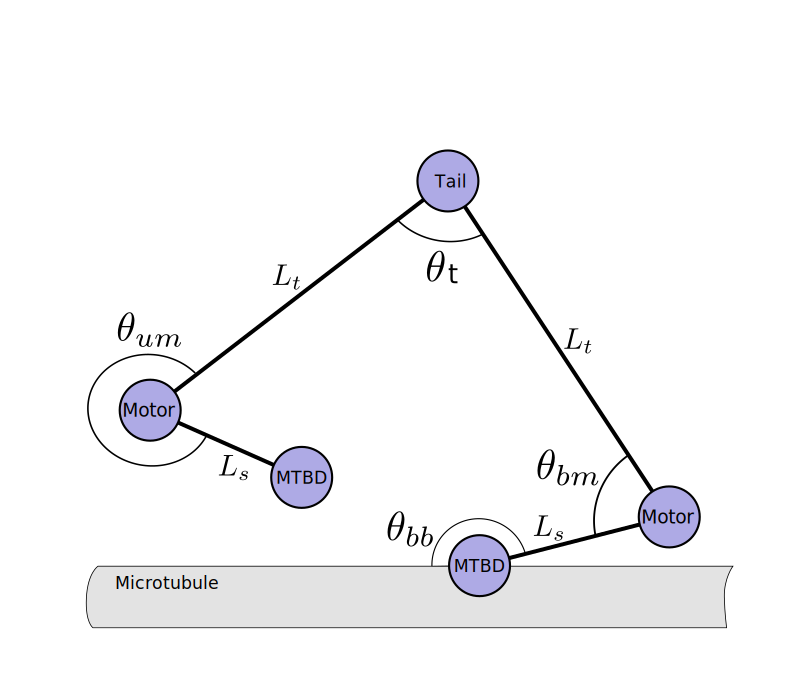
\includegraphics[width=\linewidth]{figures/schematic-1-model}
   \label{fig:explengths}
 \end{minipage}
 %
 \begin{minipage}{.3\textwidth}
   \centering
   \includegraphics[width=\linewidth]{figures/schematic-2-cryoem}
   \label{fig:modlengths}
 \end{minipage}%
 \begin{minipage}{.3\textwidth}
   \centering
   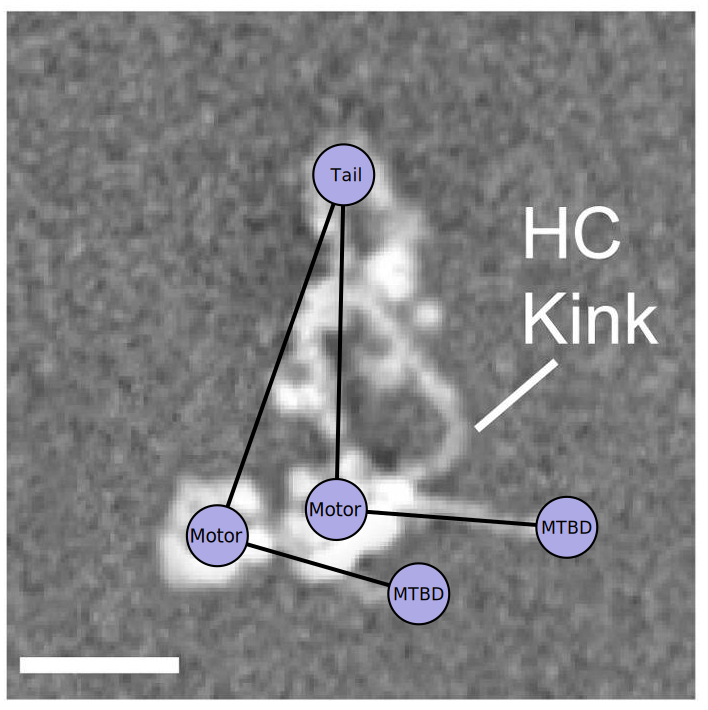
\includegraphics[width=\linewidth]{figures/schematic-2-superimposed}
   \label{fig:modlengths}
 \end{minipage}%
 \begin{minipage}{.3\textwidth}
   \centering
   \includegraphics[width=\linewidth]{figures/schematic-2-model}
   \label{fig:explengths}
 \end{minipage}
\caption{\textbf{Model schematic superimposed on cryo-EM images of native dynein.} Native cryo-EM images of the full dimerized dynein complex composed of light, intermediate and heavy chains, from \cite{nativestructure}. Model schematics are superimposed for illustrative purpose; shown angles to not represent expected \textit{in vivo} equilibria. Schematics are shown docked to a microtubule for illustrative purposes.}
\label{fig:modelparams}
\end{figure}

\begin{figure}%[tbhp]
\centering
 \begin{minipage}{0.5\textwidth}
   \centering
   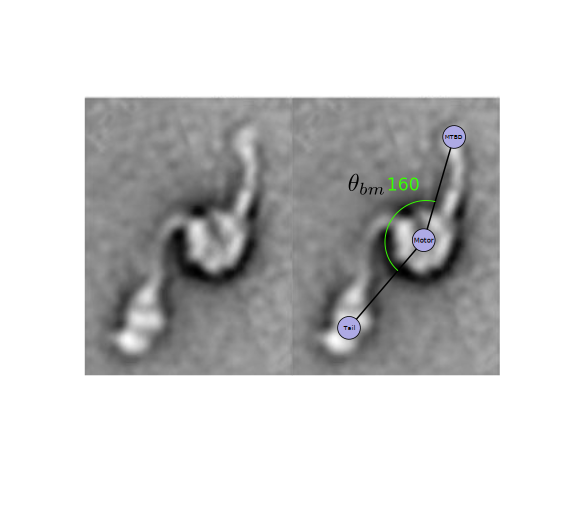
\includegraphics[width=\linewidth]{figures/schematic-prestroke}
   \label{fig:prestrokeangle}
 \end{minipage}%
 \begin{minipage}{0.5\textwidth}
   \centering
   \includegraphics[width=\linewidth]{figures/schematic-poststroke}
   \label{fig:poststrokeangle}
 \end{minipage}
 %
 \begin{minipage}{\textwidth}
   \centering
   \includegraphics[width=\linewidth]{figures/schematic-binding-angle}
   \label{fig:bindingangle}
 \end{minipage}
\caption{\textbf{Schematic of model equilibrium angles over cryo-EM images.} \textbf{a.)} Prestroke and \textbf{b.)} poststroke dynein heavy chains superimposed with model motor angles, both from \cite{burgess-paper}. \textbf{c.)} Axonemal dynein bound to MT with model binding angle superimposed, from \cite{leschziner}.}
\label{fig:modelangles}
\end{figure}



\end{document}
